\documentclass[convert={density=1200,size=400x,outext=.png}]{standalone}
\usepackage{tikz}
\usetikzlibrary{arrows.meta,calc,shadings}
\pagestyle{empty}
\begin{document}
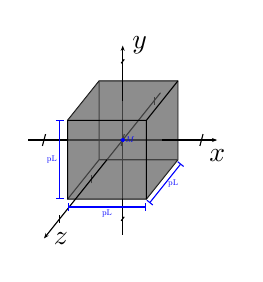
\begin{tikzpicture}[x={(1cm,0)},y={(0,1)},z={(-0.4cm,-0.5cm)},>={Stealth[scale=.4]}]
  % Achsen
  \draw (-1.2,0,0)--(.5,0,0);
  \draw (0,-1.2,0)--(0,.5,0);
  \draw (0,0,-1.2)--(0,0,.5);
  % Skalenstriche
  \draw \foreach\x in {-1,...,1} { (\x,-.05,.05)--(\x,.05,-.05) };
  \draw \foreach\y in {-1,...,1} { (0,\y,-.05)--(0,\y,.05) };
  \draw \foreach\z in {-1,...,2} { (0,-.05,\z)--(0,.05,\z) };
  \draw (-.5,.5,.5) -- (-.5,.5,-.5) (-.5,-.5,.5) -- (-.5,-.5,-.5) (.5,-.5,.5) -- (.5,-.5,-.5)
  (-.5,-.5,-.5) rectangle (.5,.5,-.5);
  \fill[fill=black!64,fill opacity=.7]  (-.5,-.5,.5) -- (-.5,.5,.5) -- (-.5,.5,-.5) -- (.5,.5,-.5) -- (.5,-.5,-.5) -- (.5,-.5,.5) -- cycle;
%  \fill[fill=black!40,fill opacity=.5] (-.5,-.5,.5) rectangle (.5,.5,.5);
%  \fill[fill=black!40,fill opacity=.5] (-.5,-.5,.5)--(-.5,-.5,-.5)--(-.5,.5,-.5)--(-.5,.5,.5)--cycle;
%  \fill[fill=black!40,fill opacity=.5] (.5,-.5,.5)--(.5,-.5,-.5)--(.5,.5,-.5)--(.5,.5,.5)--cycle;
%  \fill[fill=black!40,fill opacity=.5] (-.5,.5,.5)--(.5,.5,.5)--(.5,.5,-.5)--(-.5,.5,-.5)--cycle;
  \draw (-.5,-.5,.5) rectangle (.5,.5,.5) (.5,.5,.5) -- (.5,.5,-.5);
  % draw last part of the z-axis
  \draw[->] (0,0,.5)--(0,0,2.5) node[right]{$z$};
  \draw[->] (0,.5,0)--(0,1.2,0) node[right]{$y$};
  \draw[->] (.5,0,0)--(1.2,0,0) node[below]{$x$};
  \draw[blue] plot[scale=.2,mark=*] (0,0,0) node[scale=.3,right]{$M$};
  \draw[blue,<->,>={Bar[scale=.6]}] (-.5,-.6,.5) -- node[scale=.3,below]{pL} (.5,-.6,.5);
  \draw[blue,<->,>={Bar[scale=.6]}] (-.6,.5,.5) -- node[scale=.3,left]{pL} (-.6,-.5,.5);
  \draw[blue,<->,>={Bar[scale=.6]}] (.54,-.55,.5) -- node[scale=.3,right]{pL} (.54,-.55,-.5);
%  \draw[blue,<->, >={Bar[scale=.6]},shift={(-.05cm,.05cm)}] (0,0,1)--(0,0,-1) node[above,sloped,scale=.3,pos=.65] {pHoehe};
\end{tikzpicture}
\end{document}